\documentclass[leqno]{article}
\usepackage[margin=0.5in]{geometry}
\usepackage[utf8]{inputenc}
\usepackage{amsmath, amsfonts, color, booktabs, centernot, graphicx, fancyhdr}
\usepackage[linktoc=all,hidelinks]{hyperref}
\setlength\parindent{0pt}
\begin{document}
\title{Markov Chain Model of Genetic Evolution: EE 126 Project 1}
\author{Ajeya Cotra, Leah Dickstein, Davis Foote, Ena Hariyoshi}

\maketitle
 
\setlength{\parskip}{\baselineskip}

Our project uses a Markov chain to model the genetic evolution of the peppered moth ({\it Biston betularia}) over the last two hundred years.

\section{Background}

The dramatic changes the species underwent in a relatively short evolutionary time span make the peppered moth one of the most well-studied and celebrated creatures in evolutionary biology. {\it Biston betularia}, native to England, started off mostly white, to camouflage with the light trees and lichen in its environment:

\begin{center}
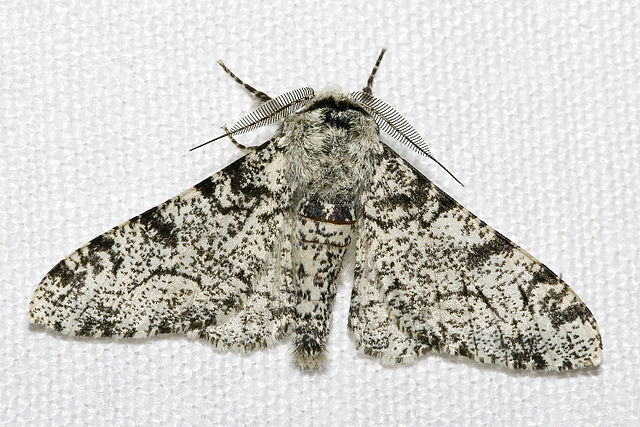
\includegraphics[scale=0.8]{white_peppered_moth.jpg}{\\White peppered moth, {\it Biston betularia f. typica}.}
\end{center}

However, with the advent of the industrial revolution, increased pollution in the moths' habitats killed off most lichen and stained light-colored trees with soot, causing white moths to stand out against the darkened environment. The previously advantageous coloring now made lighter moths more visible to predators. Over the next several decades, white peppered moths were almost completely eliminated from the population and {\it Biston betularia} became dark gray colored:

\begin{center}
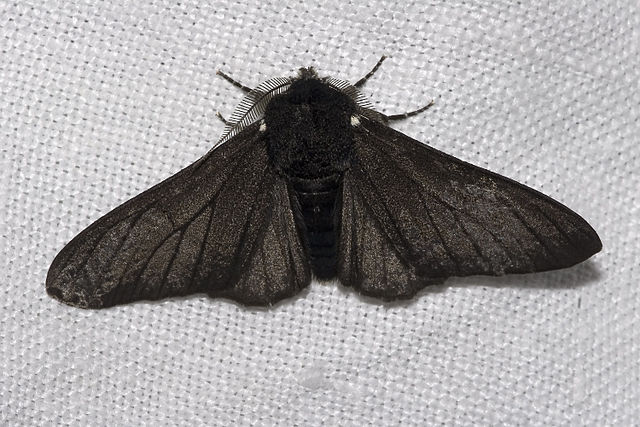
\includegraphics{black_peppered_moth.jpg}{\\Black peppered moth, {\it Biston betularia f. carbonaris}.}
\end{center}

The white peppered moth was virtually eliminated from the population in a very short time. This led us to wonder what evolutionary pressure would be necessary to have a high probability of fully eliminating a trait from a population within a fixed amount of time.

\newpage

\section{Simulation}

In our simulation, individual moths are either white or gray. Coloration is modeled as a Mendelian trait -- two alleles, $W$ and $g$, represent the white and gray traits respectively. Each moth has two color alleles which together determine its color. In our model, white is dominant, so $WW$ and $Wg$ mean the moth is white, while $gg$ means the moth is gray.

We model a moth population as a discrete time Markov chain whose states represent the number of $WW$, $Wg$, and $gg$ moths in the population (for example, in an experiment with population $45$, the state may record $15$ $WW$ moths, $23$ $Wg$ moths, and $7$ $gg$ moths at time $k$). At each time step, the population experiences exactly one birth and one death, detailed in the transition model below.

\subsection{Transition Model}

Let $N$ be the total number of moths in the population. Because at each time step we have exactly one birth and one death, $N$ remains stable. Define $N_{ww}$ to be the number of $WW$ moths, $N_{wg}$ to be the number of $Wg$ moths, and $N_{gg}$ to be the number of $gg$ moths. At time $k$, our state $X_k$ is represented as $\{N_{ww},\ N_{wg},\ N_{gg}\}$. 

\textbf{Birth}

To transition, we begin with the birth phase. Two moths are chosen at random from the current population. One allele is randomly selected from each parent to produce an offspring moth. The probability of each offspring genotype given parent genotypes are given in the table below:

\begin{tabular}{c|c|c|c|c|c|c|} \cline{2-7} 
{} & \multicolumn{6}{|c|}
{Parent genotypes}\\
\hline
\multicolumn{1}{|c|}{Offspring genotype} & WW, WW & WW, Wg & WW, gg & Wg, Wg & Wg, gg & gg, gg\\
\hline
\multicolumn{1}{|c|}{WW} & 1 & 1/2 & 0 & 1/4 & 0 & 0\\
\multicolumn{1}{|c|}{Wg} & 0 & 1/2 & 1 & 1/2 & 1/2 & 0\\
\multicolumn{1}{|c|}{gg} & 0 & 0 & 0 & 1/4 & 1/2 & 1\\
\hline
\multicolumn{1}{|c|}{Total} & $\left(\frac{N_{ww}}{N}\right)^2$ & $2\left(\frac{N_{ww}}{N}\right)\left(\frac{N_{wg}}{N}\right)$ & $2\left(\frac{N_{ww}}{N}\right)\left(\frac{N_{gg}}{N}\right)$ & $\left(\frac{N_{wg}}{N}\right)^2$ & $2\left(\frac{N_{ww}}{N}\right)\left(\frac{N_{gg}}{N}\right)$ & $\left(\frac{N_{gg}}{N}\right)^2$ \\
\hline
\end{tabular}\\

Let $b_x$ be the probability that the offspring moth created has genotype $x$. From the table above we can calculate 

\begin{align*}
% b_{ww} &= \left\left(\frac{WW}{N} \right\right)^2 + \frac{WW\, gg}{N^2} + \frac{1}{4}\left\left(\frac{wg}{N}\right\right)^2\\
b_{ww}\ &=\ \frac{1}{N^2}\left((WW)^2\ +\ (WW)\, (gg)\ +\ \frac{1}{4}\, Wg\right)\\
% b_{wg} &= \frac{WW\, Wg}{N^2} + \frac{1}{2}\left\left(\frac{Wg\, gg}{N^2}\right\right) + \frac{1}{2}\left\left(\frac{Wg}{N}\right\right)^2 + 2\, \frac{WW\, gg}{N^2}\\
b_{wg}\ &=\ \frac{1}{N^2}\left( (WW)\, (Wg)\ +\ \frac{1}{2}\, (Wg)\, (gg)\ +\ \frac{1}{2}\, (Wg)^2\ +\ 2\, (WW)\, (gg) \right)\\
b_{gg}\ &=\ \frac{1}{N^2}\left((gg)^2\ +\ (gg)\, (Wg)\ +\ \frac{1}{4}\, (Wg)^2\right)
\end{align*}

Once a moth is born, we update $N$ and the appropriate count ($WW$, $Wg$, or $gg$) to reflect this.\\

\textbf{Death}

Following the birth of the offspring moth, we randomly select a moth from the entire population (including the new offspring) to kill before we transition to the next time step. The state at $k + 1$ will be the resulting count of $WW$, $Wg$, and $gg$ after {\it both} one birth and one death have occurred.

\newpage

Probability of death is determined by {\it phenotype} rather than genotype: a white moth has probability $d_{white}$ of death. Let $d_x$ be the probability that a moth of genotype $x$ is chosen to be killed. We can calculate the $d_x$ in terms of $d_{white}$ from the information above:

\begin{align*}
d_{ww}\ &=\ d_{white}\, P(WW \mid \text{white})\ &=\ d_{white}\, \left(\frac{WW}{WW\ +\ Wg}\right)\\
d_{wg}\ &=\ d_{white}\, P(Wg \mid \text{white})\ &=\ d_{white}\left(\frac{Wg}{WW\ +\ Wg}\right)\\
d_{gg}\ &=\ 1 - d_{white}
\end{align*}

\textbf{State Transitions}

If the Markov chain is in state $X_k\ =\ \{N_{ww},\ N_{wg},\ N_{gg}\}$ where $N_{ww},\, N_{wg},\ N_{gg}\ >\ 0$, then based on the birth and death in that state, there are $7$ possibilities for state $X_{k + 1}$: 

\begin{align*}
\{N_{ww} - 1,\ N_{wg} + 1,\ N_{gg}\} &\ \implies \text{ $Wg$ born, $WW$ died}\\
\{N_{ww} - 1,\ N_{wg},\ N_{gg} + 1\} &\ \implies \text{ $gg$ born, $WW$ died}\\
\{N_{ww} + 1,\ N_{wg} - 1,\ N_{gg}\} &\ \implies \text{ $WW$ born, $Wg$ died}\\
\{N_{ww},\ N_{wg} - 1,\ N_{gg} + 1\} &\ \implies \text{ $gg$ born, $Wg$ died}\\
\{N_{ww} + 1,\ N_{wg},\ N_{gg} - 1\} &\ \implies \text{ $WW$ born, $gg$ died}\\
\{N_{ww},\ N_{wg} + 1,\ N_{gg} - 1\} &\ \implies \text{ $Wg$ born, $gg$ died}\\
\{N_{ww},\ N_{wg},\ N_{gg}\} &\ \implies \text{ Same type born as died}
\end{align*}

If one or more of the $N_x$ is $0$, there are fewer transition possibilities. In particular, there are two absorbing states:

\begin{align*}
\{N_{ww} > 0,\ 0,\ 0\} &\ \implies \text{ Gray allele eliminated}\\
\{0,\ 0,\ N_{gg} > 0\} &\ \implies \text{ White allele eliminated}
\end{align*} 

The transition diagram below depicts the web of transitions visually for a population of size $3$:

\begin{center}
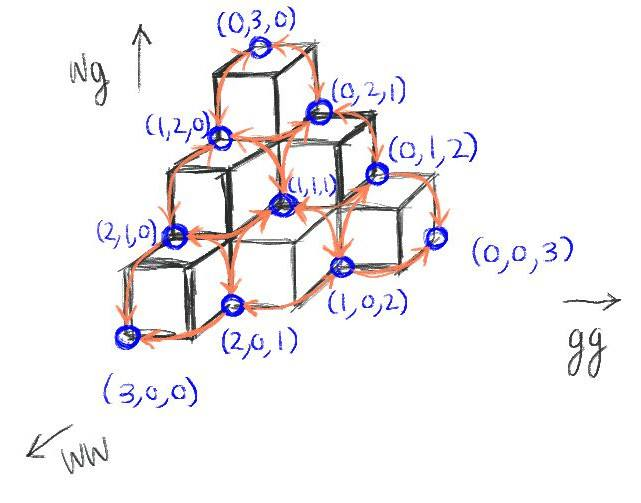
\includegraphics[width=3in]{transition_diagram.jpg}{\\States depicted in blue and transitions in orange.}
\end{center}

If transitioning into a particular state requires a moth of genotype $x$ to be born and a moth of genotype $y$ to be killed, the transition probability is simply $b_{x}\, d_{y}$.

\subsection{Python Implementation}

The project code can be found in the {\tt sim.py} file. The main function is {\tt simulate}, which simulates the change in genotype distribution over time of a given initial moth population.


\textbf{Interface}

The {\tt simulate} function takes in an {\tt initial\_state} and three optional parameters: 

\indent {\tt prob\_white}, the probability that the moth killed in a given transition is white --- defaults to {\tt 0.9} 

\indent {\tt max\_steps}, the number of time steps the program is allowed to simulate --- defaults to {\tt 10000}

\indent {\tt fraction}, a flag which indicates what to do if {\tt max\_steps} is reached before an absorbing state: if {\tt True}, it returns the fraction of gray moths left; if not, it simply returns {\tt False} to indicate white moths weren't eliminated --- defaults to {\tt True}

The {\tt simulate} function runs until it either reaches an absorbing state or has run {\tt max\_steps} times. If the population is entirely gray, it returns {\tt True}. If the population is entirely white or {\tt max\_steps}, it returns {\tt False}. If no absorbing state is reached by the end of the simulation, it returns either {\tt False} or the fraction of the population that is gray based on the value of {\tt fraction}.

\textbf{State Representation}

States are represented as Python dictionaries of length $3$. The keys are genotypes, represented by the strings {\tt `ww'}, {\tt `wg'}, and {\tt `gg'}, and the values are the number of moths of that genotype. The user must input {\tt initial\_state} in that format. Population size is inferred by summing over the values of the dictionary, and is kept constant through the simulation.

\subsection{Limitations}

This simulation provides an informative but very simplified insight into the evolutionary process. We discuss notable limitations of the model below.

First, neither our analytical model nor our simulation partitions moths into disjoint sets for mating. Both the calculations and the code make the assumption that any moth can mate with any moth. This does mean there is some probability that a moth may mate with itself. However, for larger population sizes this probability becomes negligible and does not affect the results very much.

The model assumes white moths will always die with a constant {\tt prob\_white}. A notable flaw in this model of death is that the probability that a moth of a given color will die has no dependence on the number of moths of that color; if only one white moth is left, it is extremely likely to be the one killed, which is not a very realistic assumption.

\newpage

\section{Results}

There are two interesting questions we can ask about the data. First, under what circumstances do we reliably eliminate all white moths? Second, when we don't eliminate the white allele, what fraction of the moths are now gray?

It's obvious that as {\tt prob\_white} increases, the probability that all white moths are eliminated within {\tt max\_steps} also increases. What's more interesting is the relationship between the population size and the probability that all moths turn gray. Below is a plot of the probability that all moths turn gray against population size, with {\tt prob\_white} fixed at {\tt 0.8}: 

\begin{center}
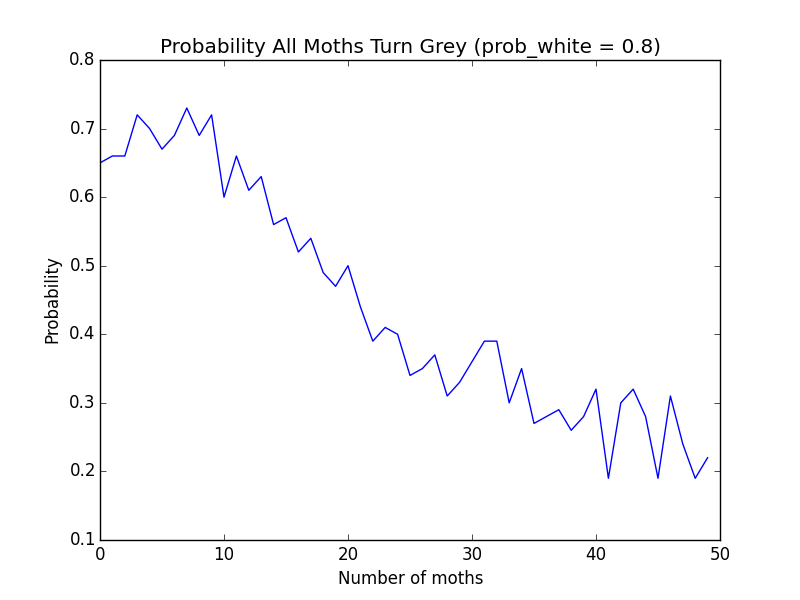
\includegraphics[width=3.7in]{all_moths_8.png} 
\end{center}

With {\tt prob\_white} equal to 0.8, as the number of moths increases, it becomes more and more difficult to fully eliminate a trait from the population.

\begin{center}
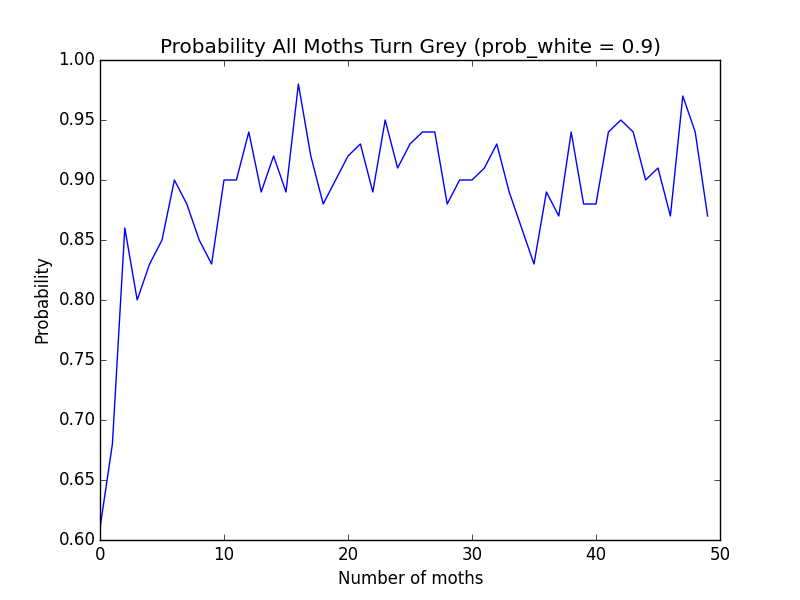
\includegraphics[width=3.7in]{all_moths_9.png} 
\end{center}

On the contrary, with {\tt prob\_white} equal to 0.9, as the number of moths increases, it becomes more likely that all the moths become grey. This suggests that between 0.8 and 0.9, there is some probability at which this plot will flatten out and we will see an equilibrium. As the probability deviates from this equilibrium, a higher population size decreases the variance of whether we see all moths turn grey, and this probability approaches either 1 or 0. 

\newpage
The above plots showed the probability of all moths turning grey. As we will see, the fraction of moths grey after the maximum number of steps is taken reflects almost the exact same trends. The plot below shows the fraction of grey moths at the end of the simulation as a function both of {\tt prob\_white} and the population size.\footnote{Fun fact: the color on this plot corresponds to the expected average color of the population of moths after the simulation.} 

\begin{center}
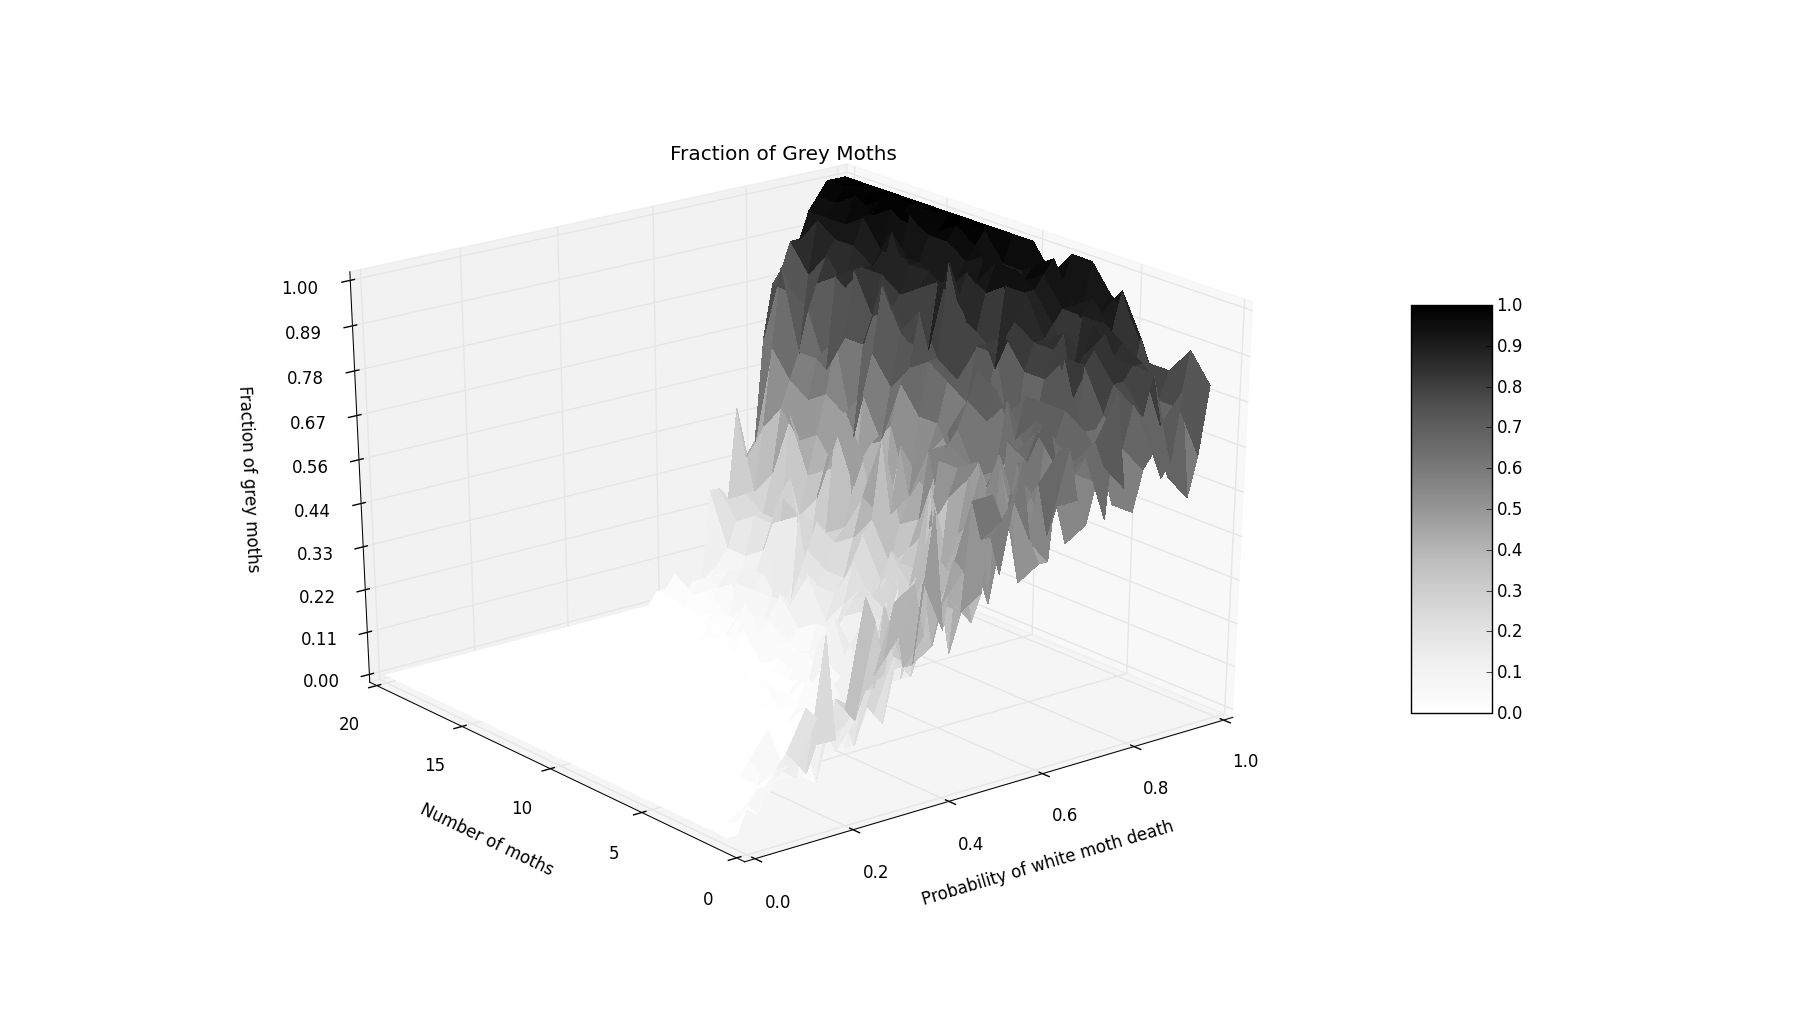
\includegraphics[width=6in]{moth_color.png}
\end{center}

We see the general trends we would expect. 

% As mentioned above, as population size increases, deviation from around the equilibrium probability (near 0.87) goes to 0 or 1 more quickly. 

As mentioned above, there is an equilibrium {\tt prob\_white} (around 0.87\footnote{This was approximated empirically by trying several projections of the 3D plot around this region.
}). Around this point, the relative frequencies of gray and white moths don't tend to change with population size. When {\tt prob\_white} is above this threshold, the system's tendency is for all moths to become gray. When it's below, the proportion of gray moths goes to $0$. 

As the population increases, the variance of the distribution of genotypes decreases. Because of low variance, large populations will tend to converge much more quickly to the tendency given by {\tt prob\_white}. This is reflected in the plot by the increase in gradient as population size increases.

This is the reason for the dip in the top-right corner; with a small population, variance is very high, so even with a very high probability of white moth death, we don't converge as quickly to an entirely gray population. Note that the two plots above are roughly projections of this 3D plot onto the planes {\tt prob\_white} = 0.8 and {\tt prob\_white} = 0.9. 

\end{document}